\section{Pre-registration history}
\label{app:prereg}

We pre-registered in four steps, in the public repository's git history, and report all four. Times are git commit times in IST (UTC+05:30).

\begin{enumerate}
  \setlength\itemsep{0pt}
  \item Commit \texttt{bf5ebe4} (2026-10-04 17:59 IST) registered hypotheses about the mechanism, a regex-only tokenizer ablation, a cross-script dose--response and from-scratch training. Our literature check then found that \citet{regmi2026vowel} had published the mechanism, the ablation, the cross-script analysis and a from-scratch downstream comparison five weeks earlier. We withdrew those hypotheses as contributions and do not report them as new.
  \item Commit \texttt{3c03367} (2026-10-04 18:16 IST), before any model was trained or evaluated, registered the retrofit study reported here: arms \RO{}, \RI{}, \RII{} and the untrained base model as a reference; $K{=}32{,}000$ unless \RII{} saturated earlier on FLORES dev; equal-bytes continued pretraining; learning rate selected once per model on \RO{}; two seeds; primary metric held-out native Nepali BPB with a non-inferiority margin of 0.01 bits per byte; English BPB as a control; Belebele, translation and decoding speed as secondary. Its compression prediction (P1), including the letters-only floors, had already been measured when it was written, so we report P1 as a measurement, not a confirmed prediction.
  \item Commit \texttt{5ff74e8} (2026-10-04 19:50 IST), amendment 2, was written after an internal review and before any continued-pretraining run had produced an evaluation. Earlier launches of continued pretraining were stopped by us before completion because of pipeline bugs, and none produced an evaluated checkpoint. The only evaluation run before the amendment, of the untouched base Llama-3.2-1B with a since-fixed document-prefix bug, is discarded. The amendment fixed the primary analysis as stated in \S\ref{sec:setup}.
  \item Commit \texttt{bfab80d} (2026-10-04 21:46 IST), amendment 3, was written \emph{after} observing Experiment A's Llama \RO{} and \RII{} results and before any \RI{} or Qwen result. It registered Experiment B (embedding warm-up, more data) and added a `worse' category to the claim rules. We report all comparisons under amendment 2's rules, which do not use that category.
\end{enumerate}

\paragraph{Deviations from the second registration (amendment 2).}
\begin{itemize}
  \setlength\itemsep{0pt}
  \item Qwen3-0.6B-Base replaces Qwen3-1.7B-Base (budget and time; same tokenizer).
  \item 1\,GB of Nepali and 1\,GB of English per arm replace 3\,GB and 3\,GB, with identical documents in every arm.
  \item A fixed learning rate of $10^{-4}$ for every run replaces selection on \RO{} from $\{3{\times}10^{-5}, 10^{-4}, 3{\times}10^{-4}\}$ by a 200-step pilot, which was never completed.
  \item One seed (seed 0) per arm replaces two.
  \item New: \RO{} and \RI{} are also checkpointed at \RII{}'s final step count (equal-compute view).
  \item New: byte-matched BPB on pieces of about 2{,}000 bytes is the primary metric; the registered sliding-window BPB becomes secondary.
  \item New: a paired bootstrap over held-out pieces, with explicit claim rules, is the primary test.
  \item The translation cap is 512 new tokens instead of 256, to avoid truncating Nepali output of \RO{}.
\end{itemize}

\paragraph{Pipeline bugs fixed before any reported run.} (1) Documents had been stored one per line with their internal newlines, so ``documents'' were paragraphs; they are now stored as one JSON-encoded document per line. (2) New-token embeddings had been initialised by decoding tokens to text, which turns partial UTF-8 tokens into U+FFFD; constituents now come from applying the original merges to the byte-level string. (3) The initialisation exactness check had covered Qwen's padding rows; it now covers only the original vocabulary. (4) Evaluation had prefixed documents with end-of-text, while base Llama expects its beginning-of-sequence token; we now use the latter where it exists, identically for every arm of a model.

Between the first two commits, the retrofit tokenizer code was tested on a 30\,MB sample of the FineWeb-2 Nepali \emph{test} split only.

\section{Repair details}
\label{app:regex}

\paragraph{Regex edit.} For the Llama-3/Qwen pattern the word branch changes as follows:
\begin{center}\small
\texttt{[\textasciicircum\textbackslash r\textbackslash n\textbackslash p\{L\}\textbackslash p\{N\}]?\textbackslash p\{L\}+}\\
$\downarrow$\\
\texttt{[\textasciicircum\textbackslash r\textbackslash n\textbackslash p\{L\}\textbackslash p\{M\}\textbackslash p\{N\}]?[\textbackslash p\{L\}\textbackslash p\{M\}]+}
\end{center}
and the same change is made in the punctuation branch \texttt{\textvisiblespace?[\textasciicircum\textbackslash s\textbackslash p\{L\}\textbackslash p\{N\}]+}. The optional leading class and the punctuation class must exclude \pM{}, so that a mark can only be matched by the word class and stays in one pre-token with the letters around it. Nothing else in the pattern changes.

\paragraph{Continued BPE.} At inference, BPE applies the lowest-ranked applicable merge first, so the original merges act before the new ones. The extended tokenizer reproduces the training procedure except in two cases: a new merge whose output string is already in the original vocabulary can let an original merge fire again afterwards, and under HuggingFace's \texttt{ignore\_merges} option (set for Llama-3) a pre-token that is itself a vocabulary entry is emitted directly. Neither case affects Proposition~\ref{prop:lossless}. We run the merge learning inside the HuggingFace Rust trainer by mapping each base token to a private-use code point. Learning $K{=}32{,}000$ merges on 1\,GB of Nepali text takes 1.7 to 3.4 minutes per tokenizer.

\paragraph{Scope of Proposition~\ref{prop:lossless}.} The proposition covers ASCII English and code, and every other script whose normalised text has no combining marks, including most Cyrillic, Han, Hangul and Ethiopic text. It does not cover Devanagari, even without marks: mark-free Devanagari words and Devanagari digits contain code points in U+0900--U+097F and change by design, since new merges apply to them. It also does not cover text with marks, such as Hindi or Latin written in decomposed form (NFD, e.g.\ \emph{caf\'e} with a combining acute). The Llama-3 tokenizer has no normalizer, so NFD input to a deployed Llama-3 \RII{} model falls outside the guarantee; Qwen3's tokenizer applies NFC itself, which composes most, but not all, combining marks. We normalise all our text to NFC. Empirically, \RI{} and \RII{} at $K{=}32{,}000$ give token ids identical to the original tokenizer on all 1{,}012 FLORES devtest sentences in English, Russian and Amharic, for both models. One Russian sentence contains a combining acute (U+0301) and so lies outside the proposition; its ids are nonetheless identical.

\paragraph{Embedding initialisation.} A new token's constituents come from applying the original merges to its byte-level string. We do not decode it to text, which would turn tokens ending in a partial UTF-8 sequence into U+FFFD. On any input whose ids are all original, the resized model produces the same hidden states, and the same logits for every original token, as the base model.

\section{Proof of Proposition~\ref{prop:lossless}}
\label{app:proof}

\begin{proof}
\emph{Pre-tokens.} The repaired regex differs from the original only in the three classes edited above, and each edited class differs from its original only on \pM{} characters. A regex match on $s$ consults only characters of $s$, and the order of the alternatives is unchanged. Since $s$ has no \pM{} character, both regexes produce the same pre-tokens.
\emph{Merges and vocabulary.} \RII{} differs from the original tokenizer only by appended merges and by the vocabulary entries they create, each of which contains a complete code point in U+0900--U+097F. A merge $(a,b)$ applies only where $a$ and $b$ are adjacent symbols of a pre-token, so its output is a contiguous substring of that pre-token's bytes. A vocabulary entry is emitted directly under \texttt{ignore\_merges} only if it equals the whole pre-token. Neither can happen for a pre-token of $s$, because UTF-8 is self-synchronising and $s$ contains no such code point. Each pre-token of $s$ is therefore encoded with original merges and original vocabulary entries only, exactly as by the original tokenizer.
\emph{Ids.} New ids are appended above the original ids, so all ids coincide.
\end{proof}

\section{Training and evaluation protocol}
\label{app:protocol}

\paragraph{Data.} We normalise to NFC, drop documents under 200 characters, remove exact duplicates, and drop every document that shares a whitespace 10-gram with FLORES-200 dev or devtest in Nepali or English. This also covers the Belebele passages, which are FLORES passages~\citep{bandarkar-etal-2024-belebele}, but not its questions or answers. Documents are stored one JSON-encoded document per line, so internal newlines are kept within a document. Before training, a 30\,MB held-out slice of each language is carved from the cleaned stream and never trained on. The 1\,GB of Nepali text used to learn merges is taken from the start of the training stream. Statistics are in Appendix~\ref{app:data}.

\paragraph{Continued pretraining.} Documents are interleaved by document and separated by the model's end-of-text token. We report each arm's training FLOPs. Optimisation is identical across arms: sequence length 2{,}048, global batch 256 sequences (0.52M tokens), AdamW ($\beta = (0.9, 0.95)$, weight decay 0.1), gradient clipping at 1.0, 1\% linear warm-up, then cosine decay to 10\% of peak, bf16 autocast with fp32 master weights, on 4$\times$H200. The peak learning rate is fixed at $10^{-4}$ for every run and is not tuned. Initialisation is deterministic and there is no dropout, so a second seed would change only the order of training windows and bf16 non-determinism.

\paragraph{Evaluation.} Every scored sequence is prefixed by the model's beginning-of-sequence token where it has one (Llama) and by its end-of-text token otherwise (Qwen), identically for every arm of a model. This is the registered prefix; \S\ref{sec:cpt} also reports a diagnostic re-scoring of held-out and FLORES BPB after the end-of-text token.
\begin{itemize}
  \setlength\itemsep{0pt}
  \item \textbf{Bits per byte (BPB)} on the held-out native Nepali and English slices (4\,MB each), and on FLORES-200 devtest. The primary metric is byte-matched BPB: each held-out document is split at whitespace into pieces of about 2{,}000 bytes, and every piece is scored independently, so every arm conditions on the same bytes of context. Token windows would give \RII{} more bytes of context per scored token. As a secondary metric, whole documents are scored with a sliding window of 2{,}048 tokens and stride 1{,}024.
  \item \textbf{Belebele}~\citep{bandarkar-etal-2024-belebele} \texttt{npi\_Deva} and \texttt{eng\_Latn}, zero-shot, scoring each of the four answer strings by its log-likelihood per byte given passage and question. Letter-choice prompting puts a 1B model at chance in both languages~\citep{regmi2026arkios}.
  \item \textbf{Translation}: FLORES-200 devtest Nepali$\leftrightarrow$English, 5-shot from FLORES dev, greedy decoding capped at 512 new tokens, chrF++.
  \item \textbf{Generation speed}: UTF-8 bytes generated per second in greedy continuation of FLORES dev Nepali sentences.
\end{itemize}
The equal-compute checkpoints are scored on BPB only, on the first 1\,MB of each held-out slice.

\section{Data}
\label{app:data}

\begin{table}[t]
\centering\small
\setlength{\tabcolsep}{3.5pt}
\begin{tabular}{lrr}
\toprule
& Nepali & English \\
\midrule
documents read & 170,790 & 215,961 \\
dropped: under 200 chars & 0 & 0 \\
dropped: exact duplicate & 0 & 69 \\
dropped: FLORES 10-gram & 0 & 16 \\
training documents & 166,300 & 209,713 \\
held-out (MB) & 30 & 30 \\
\midrule
\multicolumn{3}{l}{CPT tokens per arm (millions), 1\,GB + 1\,GB}\\
Llama-3.2-1B R0 & 207 & 211 \\
Llama-3.2-1B R1 & 176 & 211 \\
Llama-3.2-1B R2 & 76 & 211 \\
Qwen3-0.6B R0 & 359 & 215 \\
Qwen3-0.6B R1 & 177 & 215 \\
Qwen3-0.6B R2 & 76 & 215 \\
\bottomrule
\end{tabular}
\caption{Corpus cleaning (FineWeb-2 \texttt{npi\_Deva}; FineWeb-Edu; documents placed in the 30\,MB held-out slice are not counted as training documents) and the token counts of each arm's identical 2\,GB training stream. English token counts differ across arms of a model by less than 0.012\%, from the few English documents that contain Devanagari or combining marks.}
\label{tab:data}
\end{table}


\section{Full audit}
\label{app:audit}

Table~\ref{tab:audit-full} lists every distinct tokenizer. Aliases are tokenizers whose token counts are identical to another tokenizer's on all 36 FLORES languages we measured; we did not compare token ids. Kimi-K3 (requires executing remote code) and Mistral-Large-3 (degenerate HuggingFace load) are not included.

\begin{table*}[t]
\centering\small
\setlength{\tabcolsep}{4pt}
\begin{tabular}{lllrrrrrl}
\toprule
Tokenizer & Aliases & Regex & $|V|$ & ne/en & 95\% CI & Floor & Mark-init. & Lossless \\
\midrule
IndicBERTv2 & -- & none & 250,000 & 1.09 & [1.08, 1.10] & -- & 6\% & no \\
Arkios & -- & mark-aware & 65,536 & 1.12 & [1.10, 1.13] & 0.78 & 15\% & yes \\
XLM-R & -- & none & 250,002 & 1.12 & [1.11, 1.14] & -- & 7\% & no \\
NLLB-200 & -- & none & 256,204 & 1.17 & [1.16, 1.18] & -- & 6\% & no \\
BLOOM & -- & other & 250,680 & 1.18 & [1.16, 1.19] & -- & 17\% & yes \\
mT5 & -- & none & 250,100 & 1.46 & [1.45, 1.47] & -- & 11\% & no \\
Gemma-3 & Gemma-4 & none & 262,145 & 1.53 & [1.51, 1.54] & -- & 9\% & yes \\
Sarvam-1 & -- & none & 68,096 & 1.54 & [1.52, 1.56] & -- & 14\% & yes \\
o200k & gpt-oss & mark-aware & 200,019 & 1.61 & [1.60, 1.63] & 0.80 & 26\% & yes \\
Llama-4 & -- & mark-aware & 201,135 & 1.83 & [1.81, 1.85] & 0.80 & 30\% & yes \\
Mistral-NeMo & Sarvam-M & mark-aware & 131,072 & 2.13 & [2.11, 2.15] & 0.79 & 33\% & yes \\
Gemma-2 & -- & none & 256,000 & 2.13 & [2.11, 2.15] & -- & 19\% & yes \\
Qwen3.5 & -- & mark-aware & 248,077 & 2.20 & [2.18, 2.23] & 0.80 & 19\% & yes \\
Llama-3 & SmolLM3 & letters-only & 128,256 & 2.58 & [2.55, 2.61] & 2.19 & 55\% & yes \\
TituLLM & -- & mark-aware & 170,497 & 2.60 & [2.57, 2.63] & 0.78 & 55\% & yes \\
DeepSeek-V3 & DeepSeek-V4 & mark-aware & 128,815 & 2.97 & [2.93, 3.00] & 0.78 & 38\% & yes \\
GLM-5.3 & -- & letters-only & 154,856 & 4.35 & [4.29, 4.40] & 2.19 & 33\% & yes \\
Qwen2.5 & Qwen3 & letters-only & 151,665 & 4.42 & [4.36, 4.47] & 2.17 & 32\% & yes \\
Mistral-7B & -- & none & 32,768 & 4.44 & [4.38, 4.50] & -- & 29\% & yes \\
GLM-4.5 & -- & letters-only & 151,365 & 4.76 & [4.71, 4.82] & 2.19 & 30\% & yes \\
cl100k & Phi-4, OLMo-2, Granite-4.1 & letters-only & 100,277 & 4.76 & [4.71, 4.82] & 2.19 & 30\% & yes \\
Falcon3 & -- & letters-only & 131,072 & 5.07 & [5.00, 5.14] & 3.21 & 28\% & yes \\
LFM2 & -- & letters-only & 64,400 & 5.77 & [5.70, 5.84] & 2.15 & 24\% & yes \\
GPT-2 & -- & letters-only & 50,257 & 7.55 & [7.46, 7.65] & 3.23 & 19\% & yes \\
\bottomrule
\end{tabular}
\caption{All 24 distinct tokenizers (33 released tokenizers) on FLORES-200 devtest. Aliases: tokenizers with identical token counts on all 36 FLORES languages measured. Regex: letters-only, mark-aware, other, or none (no regex pre-tokenizer). ne/en: Nepali/English token premium with 95\% paired-bootstrap interval. Floor: pre-token floor under the tokenizer's own regex, a lower bound on the premium of any vocabulary extension (letters-only and mark-aware tokenizers only). Mark-init.: share of Nepali tokens whose first character is a combining mark. Lossless: decoding reproduces the input on 200 Nepali sentences. Arkios is from \citet{regmi2026arkios}. Hugging Face repositories are listed in the released code.}
\label{tab:audit-full}
\end{table*}


\paragraph{Broken syllables.} Many Nepali tokens begin with a combining mark, which no well-formed Devanagari syllable does: 55\% of Llama-3's Nepali tokens, 32\% of Qwen3's and 30\% of \texttt{cl100k}'s. The rate does not track the regex class. Mark-aware tokenizers show similar rates (26\% for \texttt{o200k}, 55\% for TituLLM, which keeps Llama-3's merges), because BPE also splits within words.

\section{Premium decomposition}
\label{app:decomp}

We write the premium as
\begin{equation*}
\frac{|T(\text{ne})|}{|T(\text{en})|} = \underbrace{\frac{|P_{\text{rep}}(\text{ne})|}{|T(\text{en})|}}_{\text{base}} \cdot \underbrace{\frac{|P(\text{ne})|}{|P_{\text{rep}}(\text{ne})|}}_{\text{regex factor}} \cdot \underbrace{\frac{|T(\text{ne})|}{|P(\text{ne})|}}_{\text{vocabulary factor}},
\end{equation*}
where $P$ is the tokenizer's own pre-tokenizer and $P_{\text{rep}}$ is the repaired Llama-3 pattern (\S\ref{sec:method}), applied to every tokenizer. The numerator of the base term is therefore the same for all tokenizers; only the English token count varies. The base lies between $0.77$ and $0.80$ for every tokenizer, because English token counts barely differ. The regex factor is $0.98$--$1.02$ for mark-aware tokenizers, $2.77$--$2.79$ for the Llama-3/Qwen/\texttt{cl100k} pattern, and $4.06$ for the GPT-2 and Falcon3 patterns, which put every run of marks in a pre-token of its own. The vocabulary factor, tokens per pre-token, is what vocabulary extension can lower, and only down to 1.

Table~\ref{tab:decomp} shows where each tokenizer's premium comes from. For Llama-3 the vocabulary factor is $1.18$, the lowest in the audit: its 128k vocabulary already nearly covers Nepali pre-tokens, and almost all of its remaining premium is the regex factor. For Qwen and \texttt{cl100k} both factors matter. Among mark-aware tokenizers, the vocabulary factor varies from $1.43$ (Arkios, trained for Nepali) to $3.79$ (DeepSeek-V3): fixing the regex is necessary but does not by itself make a tokenizer good at Nepali. Qwen3.5's word branch is our repaired class with only the leading-character class left unchanged; \citet{land2026smallbugs} reported its change for Hindi.

\begin{table}[h]
\centering
\small
\setlength{\tabcolsep}{4pt}
\begin{tabular}{lrrrr}
\toprule
Tokenizer & Premium & Base & Regex & Vocab. \\
\midrule
GPT-2 & 7.55 & 0.80 & 4.06 & 2.34 \\
LFM2 & 5.77 & 0.78 & 2.77 & 2.68 \\
\texttt{cl100k} (+3) & 4.76 & 0.79 & 2.77 & 2.17 \\
Qwen2.5/3 & 4.42 & 0.78 & 2.79 & 2.03 \\
GLM-5.3 & 4.35 & 0.79 & 2.77 & 1.98 \\
Llama-3 & 2.58 & 0.79 & 2.77 & \textbf{1.18} \\
\midrule
DeepSeek-V3/V4 & 2.97 & 0.80 & 0.98 & 3.79 \\
Qwen3.5 & 2.20 & 0.78 & 1.02 & 2.76 \\
Llama-4 & 1.83 & 0.80 & 1.00 & 2.30 \\
\texttt{o200k} (+1) & 1.61 & 0.80 & 1.00 & 2.01 \\
Arkios & 1.12 & 0.79 & 0.99 & 1.43 \\
\bottomrule
\end{tabular}
\caption{Premium = base $\times$ regex factor $\times$ vocabulary factor, on FLORES-200 devtest, for 11 of the 15 letters-only and mark-aware tokenizers in the audit (top: letters-only; bottom: mark-aware). Arkios is from \citet{regmi2026arkios}. Vocabulary extension can only lower the last column, and not below 1.}
\label{tab:decomp}
\end{table}

\section{Cross-script sweep}
\label{app:xling}

\begin{table}[h]
\centering
\small
\setlength{\tabcolsep}{3pt}
\begin{tabular}{lr|rrr|rrr}
\toprule
& & \multicolumn{3}{c|}{Llama-3} & \multicolumn{3}{c}{Qwen3} \\
Lang. & Marks & \RO{} & \RI{} & \RII{} & \RO{} & \RI{} & \RII{} \\
\midrule
Hindi & 31\% & 2.52 & 2.38 & 1.17 & 4.42 & 2.36 & 1.16 \\
Bengali & 32\% & 5.84 & 2.29 & 1.01 & 5.03 & 2.26 & 1.00 \\
Tamil & 35\% & 7.65 & 2.67 & 1.02 & 6.11 & 2.64 & 1.02 \\
Telugu & 36\% & 8.29 & 2.45 & 1.02 & 6.99 & 2.43 & 1.01 \\
Sinhala & 28\% & 8.63 & 2.30 & 1.20 & 6.88 & 2.33 & 1.24 \\
Burmese & 50\% & 11.62 & 3.02 & 1.21 & 8.93 & 2.99 & 1.11 \\
Thai$^\dagger$ & 21\% & 2.19 & 1.49 & 0.95 & 2.55 & 1.48 & 0.88 \\
\midrule
Amharic & 0\% & 7.59 & 0.98 & 0.98 & 4.05 & 0.98 & 0.98 \\
Korean & 0\% & 1.49 & 0.98 & 0.98 & 1.63 & 0.98 & 0.98 \\
\bottomrule
\end{tabular}
\caption{Language/English token premium on FLORES-200 devtest, $K{=}32{,}000$. Marks: share of NFC code points that are combining marks. Amharic and Korean have none (control). $^\dagger$Thai is written without spaces, so whole phrases are single pre-tokens and \RI{} is not yet at its floor. For \RI{}, merge learning stopped below 32{,}000 for Tamil, Telugu, Sinhala, Burmese and Hindi (Llama) (22{,}325--31{,}815 merges), because no further merge was available under the letters-only regex.}
\label{tab:xling}
\end{table}

For each language we downloaded the FineWeb-2 \emph{test} split, normalised it to NFC, and removed documents that share a whitespace 10-gram with that language's FLORES-200 dev or devtest (for Thai, which has no spaces, we also checked 50-character overlaps and found none). The resulting merge-learning text ranges from 25\,MB (Amharic) to 361\,MB (Bengali), less than the 1\,GB used for Nepali; Sinhala and Amharic \RII{} may be limited by it. $K{=}4$k and $16$k are prefixes of one $32$k run.

The Nepali filter keeps a new merge only if its output contains a complete Devanagari character. For scripts that the base vocabularies cover poorly, many characters are themselves split into byte pieces, and this filter would drop the first byte-level merge of a character and every merge built on it (for Sinhala \RII{}, on Llama-3, only 13{,}530 of 32{,}000 merges survived). For the cross-script sweep we therefore also keep merges whose output is a byte piece of a target-script character. Such merges can only fire on target-script bytes, so the English guarantee is unaffected; we verified English token ids on all 1{,}012 sentences for every tokenizer. Hindi uses the same script as Nepali, and its new merges also change Nepali tokenization; we did not measure that interaction.

\section{Released extensions}
\label{app:released}

\paragraph{Added tokens.} The bound does not apply to strings registered as HuggingFace \emph{added tokens}, which are matched before the regex runs. SinLlama~\citep{aravinda2025sinllama} extends Llama-3 for Sinhala this way, and thereby bypasses the bound for those exact strings. Added tokens are matched greedily and do not compose with merges, so they behave differently from a merge-based extension.

\begin{table}[h]
\centering
\small
\setlength{\tabcolsep}{3pt}
\begin{tabular}{llrrr}
\toprule
Base & Lang. & Tokens/floor & Gap closed & Room \\
\midrule
Llama-3-8B & te & 1.016 & 99.3\% & 3.16$\times$ \\
Llama-3-8B & si & 1.021 & 99.3\% & 2.42$\times$ \\
Llama-3-8B & my & 1.013 & 99.5\% & 5.87$\times$ \\
Llama-3.1-8B & ta & 1.018 & 99.1\% & 3.58$\times$ \\
Llama-3.1-8B & bn & 1.020 & 98.7\% & 2.74$\times$ \\
Llama-3.1-8B & gu & 1.026 & 98.9\% & 2.52$\times$ \\
Qwen2.5-7B & si & 1.019 & 99.1\% & 2.40$\times$ \\
Qwen2.5-7B & my & 1.036 & 98.2\% & 5.72$\times$ \\
Qwen3-14B & bn & 1.019 & 98.5\% & 2.71$\times$ \\
Qwen3-14B & te & 1.027 & 98.6\% & 3.11$\times$ \\
\midrule
LFM2 (2.5) & hi & 1.068 & 95.5\% & 2.24$\times$ \\
LFM2 (2.5) & ne & 1.160 & 90.5\% & 2.77$\times$ \\
LFM2 (2.5) & bn & 1.243 & 92.4\% & 2.74$\times$ \\
LFM2 (2.5) & th & 1.819 & 87.9\% & 5.57$\times$ \\
\midrule
Llama-3.1-8B & am & 1.573 & 93.8\% & 1.00$\times$ \\
\bottomrule
\end{tabular}
\caption{Released vocabulary extensions that keep the letters-only regex, on FLORES-200 devtest of the target language. Tokens/floor: extended-tokenizer tokens divided by pre-tokens under its own regex (at least 1 by construction). Gap closed: share of the base-to-floor gap that the extension removed. Room: floor under the letters-only regex divided by floor under the repaired regex. Top block: \citet{yamaguchi2026lowres}; middle: LFM2.5~\citep{smith2026inplace}; bottom: Amharic, which has no combining marks (control).}
\label{tab:released}
\end{table}

\section{Additional tokenizer arms}
\label{app:extras}

\paragraph{Regex alone, and added tokens.} Two further arms separate the parts of \RII{}. Repairing the regex without adding merges (\RII{}, $K{=}0$) changes almost nothing: $2.61\times$ for Llama-3 (from $2.58\times$) and $4.42\times$ for Qwen3. Under the repaired regex, the old merges still tokenize Nepali words in old pieces; the regex only removes the ceiling that new merges would otherwise hit. Registering \RI{}'s new strings (31{,}999 of 32{,}000; one is a partial UTF-8 sequence) as added tokens instead of merges gives $2.35\times$ for Llama-3 and $2.19\times$ for Qwen3, no better than \RI{}. The gain of \RII{} therefore needs both the regex repair and new merges.

\paragraph{Broken syllables.} Extension under the letters-only regex makes syllable breaking worse. The share of Devanagari-bearing tokens (a slightly higher base than the all-token rate of \S\ref{sec:audit}) that begin with a combining mark rises from 57\% (Llama-3) and 33\% (Qwen3) to 67\% for both under \RI{}, because new merges can only build on mark-initial fragments. Under \RII{} it falls to 15\% and 12\%.


\begin{figure}[h]
\centering
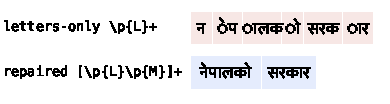
\includegraphics[width=0.95\columnwidth]{fig_split.pdf}
\caption{Pre-tokens of \emph{nep\=alko sark\=ar} (``government of Nepal'') under the letters-only regex of Llama-3 and Qwen and under the repaired regex. Dotted circles mark pre-tokens that begin with a dependent vowel sign.}
\label{fig:split}
\end{figure}

\section{All continued-pretraining runs}
\label{app:cptfull}

\begin{table*}[t]
\centering\small
\setlength{\tabcolsep}{4pt}
\resizebox{\textwidth}{!}{%
\begin{tabular}{lllrrrrrrrr}
\toprule
Model & Data & Arm & Tokens & ne BPB$\downarrow$ & en BPB$\downarrow$ & FLORES ne$\downarrow$ & Belebele ne & chrF ne$\to$en & chrF en$\to$ne & Gen.\ B/s \\
\midrule
Llama-3.2-1B & -- & base & 0 & 0.766 & 0.788 & 0.863 & 0.277 & 32.4 & 10.8 & 5327 \\
 & 1\,GB & \RO{} & 417M & \textbf{0.474} & 0.799 & 0.611 & 0.287 & 32.3 & 19.8 & 5147 \\
 & 1\,GB & \RI{} & 386M & 0.534 & 0.803 & 0.648 & 0.268 & 27.2 & 10.4 & 6354 \\
 & 1\,GB & \RII{} & 286M & 0.539 & 0.799 & 0.671 & 0.266 & 27.8 & 12.3 & 9398 \\
\addlinespace
 & 1\,GB + warm-up & \RO{} & 417M & 0.779 & 0.850 & 0.864 & 0.279 & 8.8 & 9.1 & 5349 \\
 & 1\,GB + warm-up & \RI{} & 386M & 0.808 & 0.854 & 0.904 & 0.271 & 9.9 & 4.2 & 7521 \\
 & 1\,GB + warm-up & \RII{} & 286M & \textbf{0.527} & 0.840 & 0.652 & 0.283 & 16.2 & 15.4 & 11078 \\
\addlinespace
\midrule
Qwen3-0.6B & -- & base & 0 & 0.852 & 0.873 & 0.945 & 0.290 & 26.0 & 6.8 & 2186 \\
 & 1\,GB & \RO{} & 574M & \textbf{0.501} & 0.864 & 0.631 & 0.270 & 20.1 & 13.6 & 3089 \\
 & 1\,GB & \RI{} & 392M & 0.561 & 0.864 & 0.689 & 0.253 & 11.6 & 6.9 & 4972 \\
 & 1\,GB & \RII{} & 292M & 0.570 & 0.862 & 0.688 & 0.266 & 17.0 & 3.9 & 7454 \\
\addlinespace
\bottomrule
\end{tabular}}
\caption{Continued pretraining on identical bytes per arm (one seed). BPB: bits per byte on held-out native text split into ${\sim}$2{,}000-byte pieces (primary metric) and on FLORES-200 devtest. Belebele: zero-shot accuracy (900 items, chance 0.25), scored on answer text. chrF++: 5-shot FLORES-200 devtest translation. Gen.\ B/s: UTF-8 bytes of Nepali generated per second (batch 64, greedy). Tokens: training tokens seen (for B1, excluding the embedding warm-up on the first 10\% of the same stream). Bold: best Nepali BPB within each block. All BPB here use the registered prefix; the B1 Llama rows are dominated by the scoring artifact of \S\ref{sec:cpt}, and Table~\ref{tab:prefix} gives the training-separator comparison.}
\label{tab:cpt}
\end{table*}


\paragraph{Beginning-of-sequence diagnostic.} On 40 held-out Nepali documents (first 1{,}500 characters), Llama BPB after the beginning-of-sequence token and after the end-of-text token are 0.720 and 1.865 for the base model, 0.441 and 0.438 for \RO{} of Experiment A, and 0.758 and 0.438 for \RO{} of Experiment B1. The norm of the beginning-of-sequence embedding is 0.863, 0.860 and 0.896 respectively (mean row norm 0.98--0.99).
